% done

Final states with two same-sign leptons or three leptons and multiple jets can probe a variety of supersymmetric models 
represented by decays of heavy superpartners involving massive gauge bosons, sleptons or top quarks. 
The decays of the superpartners can lead to many experimental signatures that may lead to different lepton, jet, and $b$-tagged jet multiplicities.
To exploit this wide range of possible signatures, the analysis uses six $R$-parity-conserving SUSY scenarios 
featuring gluino, bottom squark (sbottom) or top squark (stop) pair production. 
These scenarios were used as benchmarks to identify regions of the phase space 
where the analysis can bring particularly useful complementarity to other SUSY 
searches, 
and subsequently define signal regions with a particular focus on these 
regions. 
In this section, the scenarios considered are presented with details about 
the assumed superpartner masses and decay modes.  
Exclusion limits obtained prior to the work of the author will also 
be shown to highlight the improvement in reach that this analysis brings.

\begin{figure}[t!]
\centering
\begin{tabular}{rrrr}
\begin{subfigure}[t]{0.24\textwidth}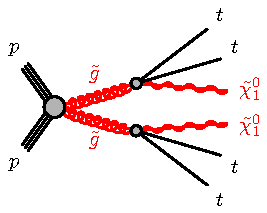
\includegraphics[width=\textwidth]{gogo-ttttN1N1}\caption{}\label{fig:strategy.pheno.feynman_gtt}\end{subfigure}&
\begin{subfigure}[t]{0.24\textwidth}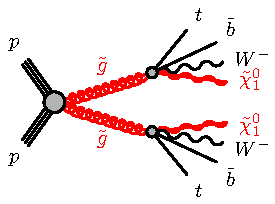
\includegraphics[width=\textwidth]{gogo-ttWWbbN1N1}\caption{}\label{fig:strategy.pheno.feynman_gttOffshell}\end{subfigure}&
\begin{subfigure}[t]{0.24\textwidth}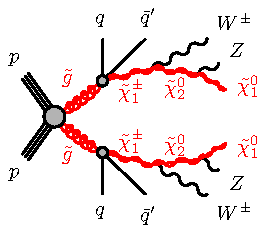
\includegraphics[width=\textwidth]{gogo-qqqqWWZZN1N1-C1N2}\caption{}\label{fig:strategy.pheno.feynman_gg2WZ}\end{subfigure}&
\begin{subfigure}[t]{0.24\textwidth}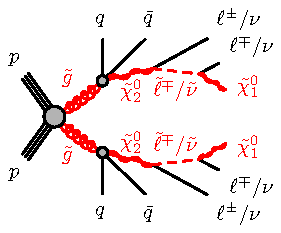
\includegraphics[width=\textwidth]{gogo-qqqqllllN1N1-N2}\caption{}\label{fig:strategy.pheno.feynman_gg2sl}\end{subfigure} \\
&
\begin{subfigure}[t]{0.24\textwidth}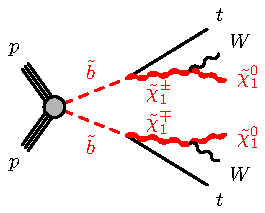
\includegraphics[width=\textwidth]{sbsb-ttWWN1N1}\caption{}\label{fig:strategy.pheno.feynman_b1b1}\end{subfigure} &
\begin{subfigure}[t]{0.24\textwidth}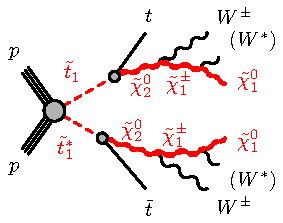
\includegraphics[width=\textwidth]{stst-ttWWWWN1N1}\caption{}\label{fig:strategy.pheno.feynman_t1t1}\end{subfigure} &
 \\
\end{tabular}
\caption{SUSY processes featuring gluino ((a), (b), (c), (d)) or third-generation squark ((e), (f)) pair production studied in this analysis. 
 In Figure~\ref{fig:strategy.pheno.feynman_gg2sl}, $\tilde{\ell} \equiv \tilde{e}, \tilde{\mu}, \tilde{\tau}$ and 
$\tilde{\nu} \equiv \tilde{\nu}_e, \tilde{\nu}_{\mu}, \tilde{\nu}_{\tau}$. In Figure~\ref{fig:strategy.pheno.feynman_t1t1}, the $W^*$ labels indicate 
largely off-shell $W$ bosons -- the mass difference between $\chinoonepm$ and $\ninoone$ is around 1~GeV.}
\label{fig:strategy.pheno.feynman}
\end{figure}


\begin{figure}[t]
\centering
\begin{subfigure}[t]{0.55\textwidth}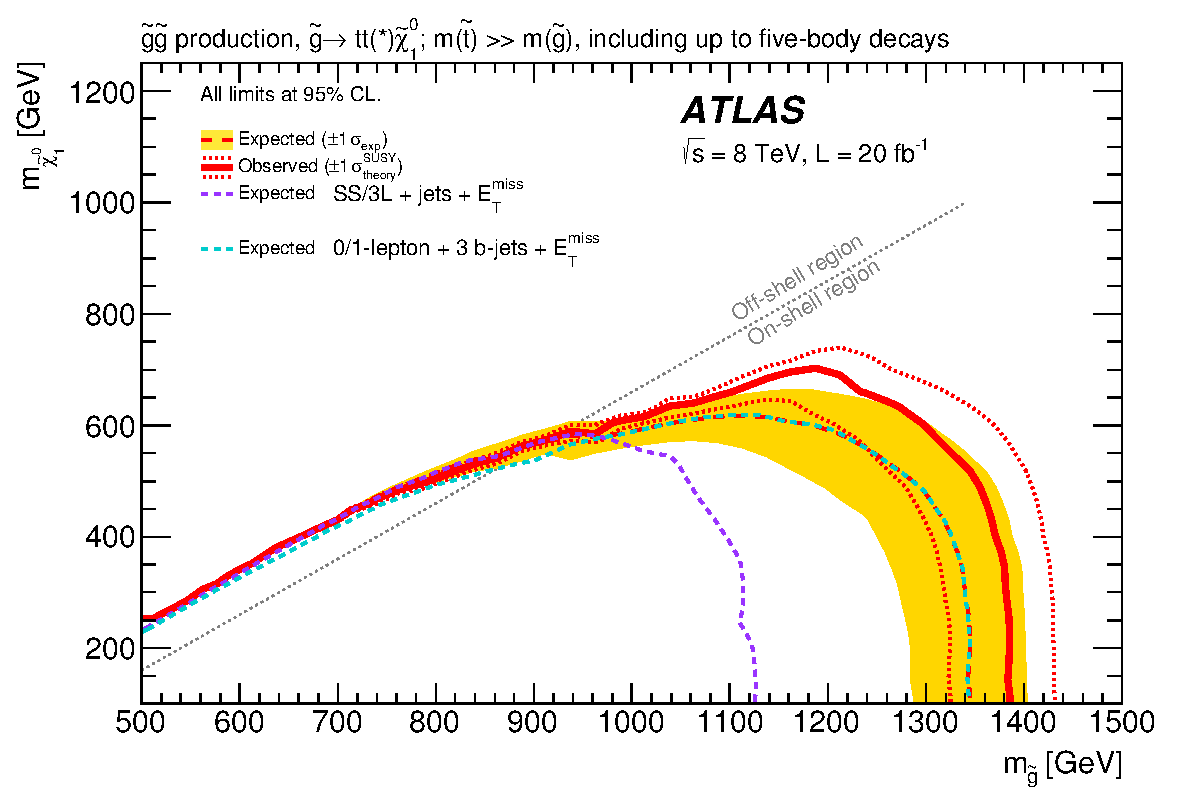
\includegraphics[width=\textwidth]{run1excluded_gluinoGtt}\caption{}\label{fig:strategy.pheno.run1_gluinoGtt}\end{subfigure}
\begin{subfigure}[t]{0.38\textwidth}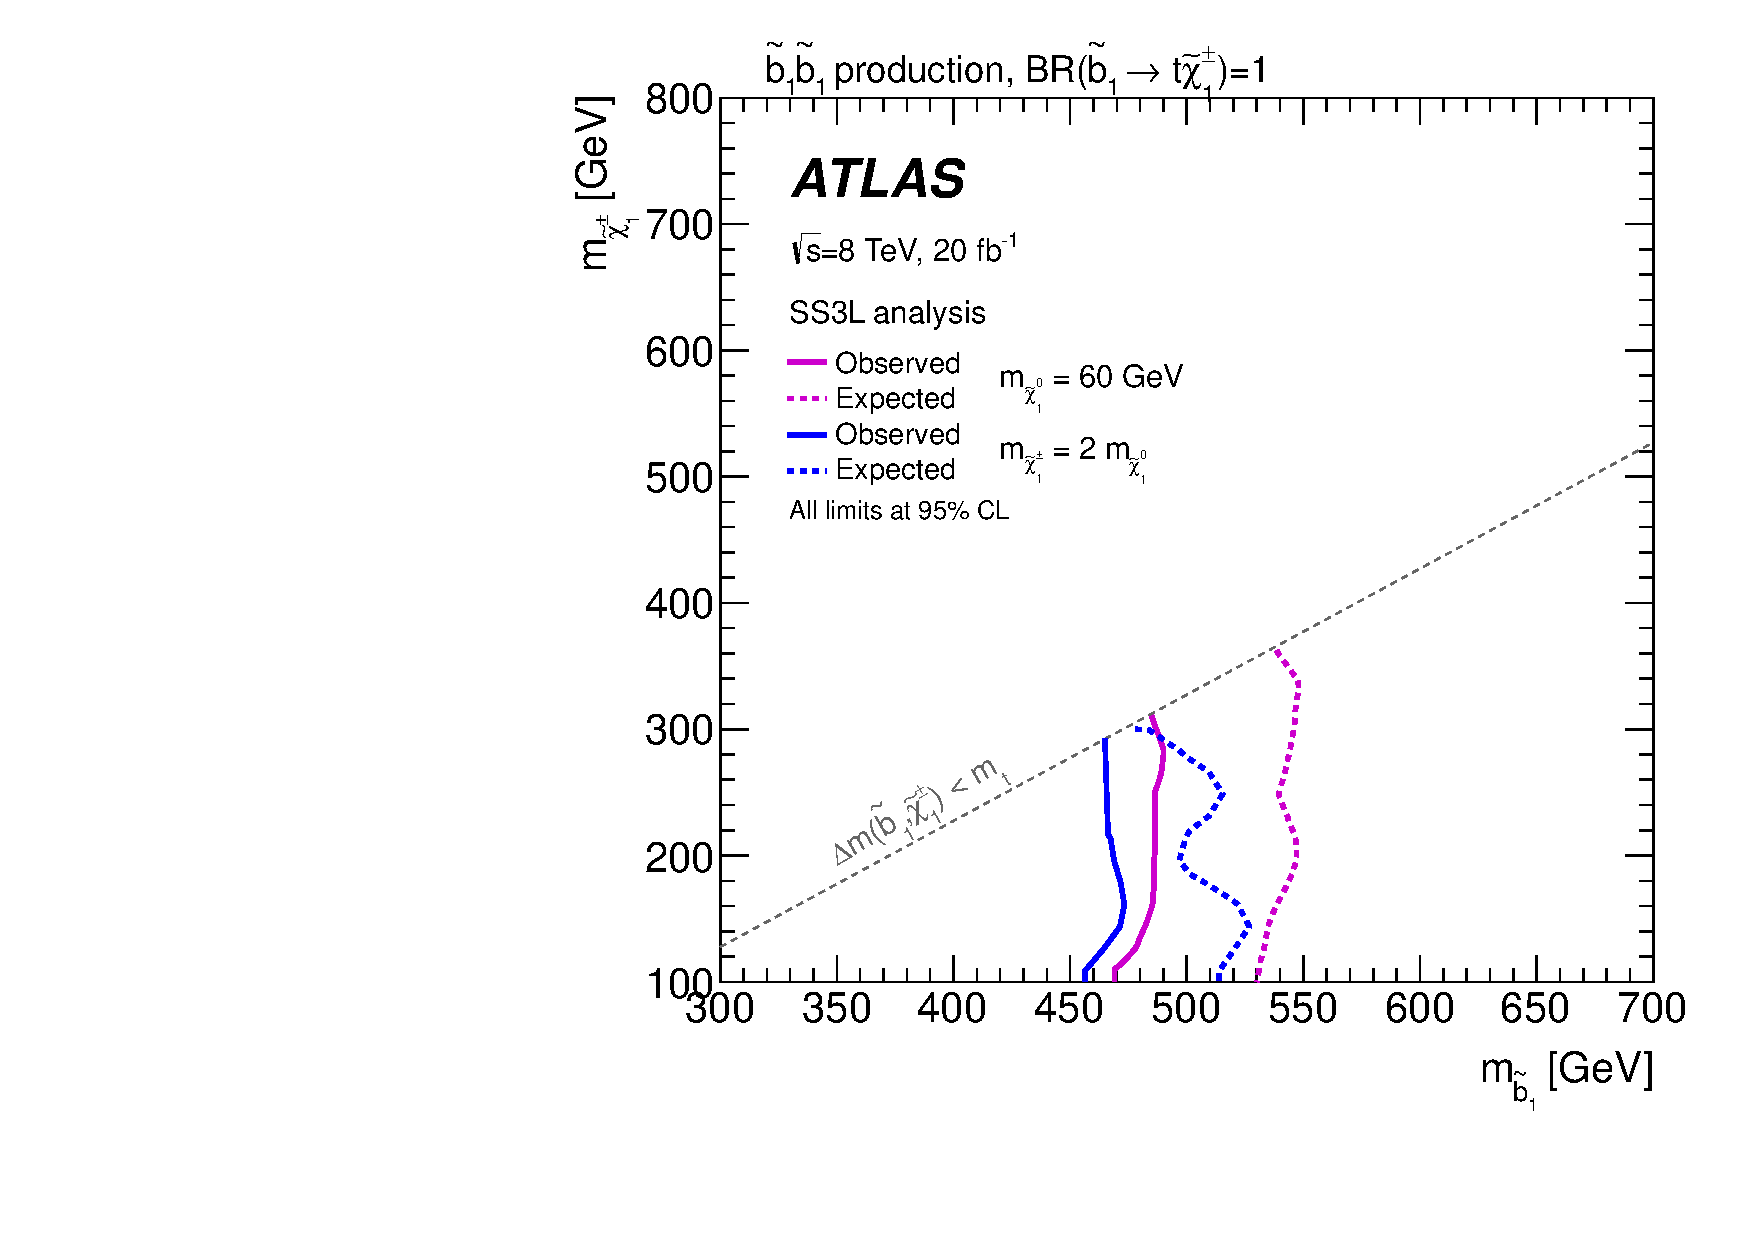
\includegraphics[width=\textwidth]{exclusion_sbottom_topC1_both_grids}\caption{}\label{fig:strategy.pheno.sbottom_topC1}\end{subfigure}
\caption{Exclusion limits on the gluino-stop offshell~\cite{SUSY-2014-06} (left) and direct sbottom~\cite{SUSY-2014-07} (right) scenarios 
set by ATLAS with the 2012 dataset prior to the author's work.}
\label{fig:strategy.pheno.run1excl_3rdgen}
\end{figure}

\begin{figure}[t]
\centering
\begin{subfigure}[t]{0.49\textwidth}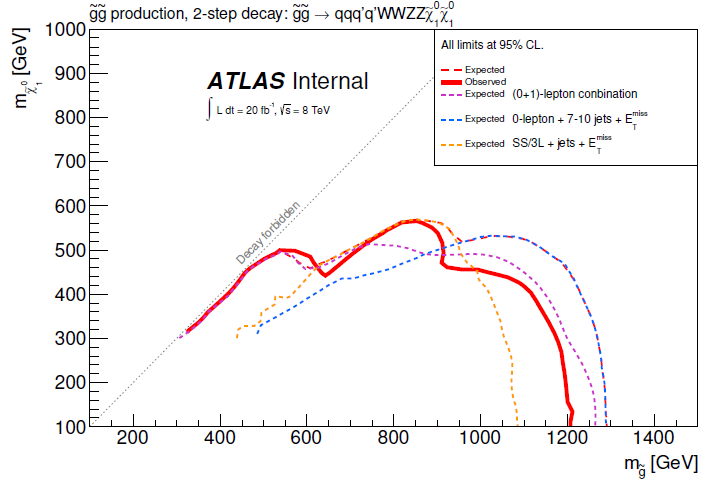
\includegraphics[width=\textwidth]{run1excluded_gluino2stepWZ}\caption{}\label{fig:strategy.pheno.run1excluded_gluino2stepWZ}\end{subfigure} 
\begin{subfigure}[t]{0.49\textwidth}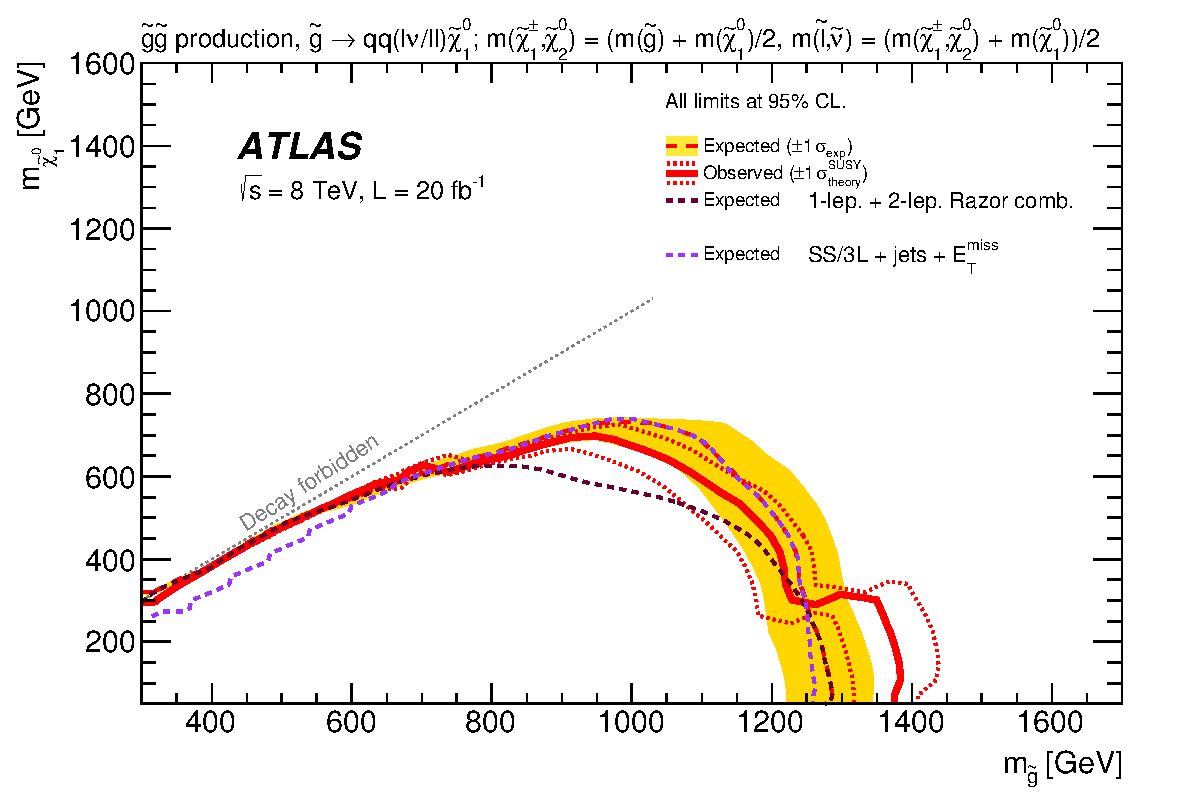
\includegraphics[width=\textwidth]{run1excluded_gluino2stepSleptons}\caption{}\label{fig:strategy.pheno.run1excluded_gluino2stepSleptons}\end{subfigure}
\caption{Exclusion limits on scenarios featuring gluino pair production followed by two-step decays via heavy gauge bosons or sleptons 
set by ATLAS with the 2012 dataset prior to the author's work~\cite{SUSY-2014-06}.}
\label{fig:strategy.pheno.run1excluded_1stgen}
\end{figure}

\subsection*{Gluino pair production with slepton-mediated two-step decay $\gl\to q\bar q\ell\bar\ell\neut$}
\label{subsec:signals_g2slep}

This scenario (Fig.~\ref{fig:strategy.pheno.feynman_gg2sl}) features gluino pair-production with two-step decays via neutralinos \neuttwo\ and sleptons, 
$\gl\to q\bar{q}'\neuttwo \to q\bar{q}'(\slep\ell/\snu\nu) \to q\bar{q}'(\ell\ell/\nu\nu)\neut$. 
The decays are mediated by generic heavy squarks, therefore the $b$-jet multiplicity in this scenario is low. 
The final state is made of charged leptons, four additional jets and invisible particles (neutrinos and neutralinos). 
The average jet multiplicity per event is the smallest among the four scenarios;  
another characteristic is the large fraction of events with several leptons, 
unlike the other scenarios that have a rather low acceptance due to the branching ratios of $W\to\ell\nu$ or $Z\to\ell\ell$. 
The exclusion limits obtained in Run 1 (Fig.~\ref{fig:strategy.pheno.run1excluded_gluino2stepSleptons}) show again that the SS/3L+jets final state 
is very competitive to probe those models. 
This scenario is used as as benchmark to define the signal regions with $\ge 3$ leptons and no $b$-jet. 

The signal grid is built with variable gluino and \neut\ masses; the \neuttwo\ mass is chosen half-way between the gluino and LSP masses, 
and the sleptons masses are also set equal and half-way between the \neuttwo\ and LSP masses. 
The \neuttwo\ may decay to any of the six ``left-handed'' sleptons (\slep, \snu) with equal probability. 
``Right-handed'' sleptons are assumed heavy and do not participate to the decay. 
%% The generated MC samples assume equiprobable mediation of the decay through all (mass-degenerate) squarks except stops, 
%% which can lead to final states with several $b$-jets in case of sbottom-mediated decays. 
%% However, we veto such decays and reweight other events by a factor $1/(2*0.2*0.8+0.2^2)$ to readjust the branching ratios, 
%% effectively modifying the model assumptions such that only decays mediated by the four light-flavour squarks occur. 
%% This is done in order to simplify the model description (the other scenario, described in the next section, doesn't have sbottom-mediated decays), 
%% as well as respect the motivation of this scenario, to be a guideline for the definition of $b$-depleted signal regions. 


\subsection*{Gluino pair production with gaugino-mediated two-step decay $\gl\to q\bar q'WZ\neut$}
\label{subsec:signals_g2wz}

This scenario (Fig.~\ref{fig:strategy.pheno.feynman_gg2WZ}) features gluino pair-production with two-step decays via gauginos and $W$ and $Z$ bosons, 
$\gl\to q\bar{q}'\chargino\to q\bar{q}'W\neuttwo\to q\bar{q}'WZ\neut$, 
mediated by generic heavy squarks of the first and second generations. 
The final state is made of two $W$ and two $Z$ bosons (possibly offshell), 
four additional jets and invisible particles (neutrinos and neutralinos). 
This generally leads to events with large jet multiplicities and a fair branching ratio for dileptonic final states. 
The exclusion limits obtained in Run 1 indeed illustrate the competitiveness of the SS/3L+jets search (Fig.~\ref{fig:strategy.pheno.run1excluded_gluino2stepWZ})
particularly the heavy-\neut\ region of the phase space. 
This scenario is used as as benchmark to define the signal regions with many jets but none tagged as a $b$-jet. 

The signal grid is built with variable gluino and \neut\ masses, 
and the \chargino\ and \neuttwo\ masses are set such that the former lies half-way between the gluino and \neut\ masses, 
and the latter half-way between \chargino\ and \neut\ masses. 

\subsection*{Sbottom pair production with one-step decay $\sbot\to t\chargino$}
\label{subsec:signals_sbot}

In this scenario (Fig.~\ref{fig:strategy.pheno.feynman_b1b1}), sbottoms are rather light and assumed to decay to a top quark and a chargino $\chargino$, 
with a subsequent $\chargino\to W^\pm\neut$ decay, 
providing complementarity to the mainstream search~\cite{ATLAS-CONF-2015-066} which focuses on the channel $\sbot\to b\neut$. 
The final state resulting from the production of a \sbsb\ pair contains two top quarks, two $W$ bosons and two neutralinos. 
While this final state may lead to various experimental signatures, 
the only model considered in Run-1~\cite{SUSY-2014-06} had
same-sign leptons and jets in the final state, leading to the exclusion limits presented in Fig.~\ref{fig:strategy.pheno.run1excl_3rdgen}. 
Signal events typically contain one or two $b$-tagged jets. 
Therefore this scenario is used as benchmark to define the signal regions with one or more $b$-jets. 

The model adopts a fixed chargino-neutralino mass difference of 100 GeV, 
which always produces on-shell $W$ bosons in the $\chargino\to W\neut$ decay
\footnote{A different chargino mass assumption is adopted in the current 
work compared to the Run 1 paper~\cite{SUSY-2014-06}.
Fig.~\ref{fig:strategy.pheno.run1excl_3rdgen} is shown for illustration only.
The reduced chargino-neutralino mass gap in the current analysis 
allows us to study signal scenarios with heavy neutralinos, which were not considered previously.}.
Only pair production of the lightest sbottom is considered, followed by an exclusive decay in the aforementioned channel. 


\subsection*{Gluino pair production with stop-mediated decay $\gl\to t\bar t\neut$}
\label{subsec:signals_gtt}

In this scenario inspired by naturalness arguments, gluinos are coupling preferentially to stops which are lighter than the other squarks. 
Gluinos are however considered lighter than stops, and decay directly into a $t\bar t\neut$ triplet via a virtual stop (Fig.~\ref{fig:strategy.pheno.feynman_gtt}). 
The pair production of gluinos leads to a final state containing four top quarks and two neutralinos. 
This characteristic final state is accessible through various experimental signatures, which is why this model 
is commonly used as a benchmark to compare analyses sensitivities. 
The searches performed with Run-1 data~\cite{SUSY-2014-06}, 
summarized in Fig.~\ref{fig:strategy.pheno.run1_gluinoGtt}, showed that the same-sign leptons final state is competitive only at large neutralino mass. 
This region of the phase space is consequently given a particular attention in the choice of signal regions described further on. 
For instance, the region of phase-space with $\Delta m(\gl,\neut)<2m_t$, where gluinos decay via one or two offshell top quarks, is only accessible for this 
analysis.
In the signal samples referenced in this document, the mass of the lightest stop is fixed to 10 \TeV~and is mostly a $\widetilde{t}_R$ state. 
Only gluino pair production is considered, followed by an exclusive decay in the aforementioned channel. 
Signal events typically contain many $b$-tagged jets, 
therefore this scenario is used as benchmark to define the signal regions with $\ge 2$ $b$-jets. 

\subsection*{\stst\ with ``three-same-sign leptons'' signature}
\label{subsec:signals_3lss}

Inspired by Ref.~\cite{Huang:2015fba}, a simplified model featuring a stop pair-production with two-step 
decays via a neutralino \neuttwo\ and a chargino $\chargino$ is added in this version of the analysis, according to the decay illustrated on 
Fig.~\ref{fig:strategy.pheno.feynman_t1t1}: \\
$\stop_1\to t \neuttwo \to t \chargino W^\mp \to t W^\pm W^\mp \neut$. 

This simplified model is a well-motivated representation of a MSSM model. 
The lightest stop ($\stop_1$) is right-handed and \neuttwo\ is bino-like 
which leads to a large branching ratio in the decay $\stop_1\to t \neuttwo$. 
Furthermore, the decay $\neuttwo \to \chargino W^\mp$ is also enhanced since $\chargino$ is wino-like, 
as long as $\chargino$ and \neut~ are nearly mass degenerate 
and $m_{\neuttwo} - m_{\neut} < m_{H} = 125$ \GeV~to suppress the decay $\neuttwo \to \neut + H$ 
(the decay $\neuttwo \to \neut + Z$ is suppressed).
By respecting these conditions and evading the bottom squark limit shown in Fig.~\ref{fig:strategy.pheno.sbottom_topC1}, we consider
 a one-dimensional grid with a $\stop_1$ mass varying between 550 \GeV~and 800 \GeV~with a 50 \GeV~gap\footnote{Only the points at $\stop_1$ mass of 550~GeV~are available at the moment.}, 
a two body decay to an on-shell top quark and a \neuttwo~ which has a 100 \GeV~mass difference from \neut.
The mass difference between the $\chargino$ and \neut~ is taken to be 500 \MeV~which is not excluded by the disappearing track 
analysis. In fact, this mass gap could easily be increased by introducing a small amount of higgsino mixing~\cite{Aad:2013di}.
%  https://atlas.web.cern.ch/Atlas/GROUPS/PHYSICS/PAPERS/SUSY-2013-01/fig_07.png

While the stop pair production is similar to the sbottom pair production in terms of kinematics, the stop pair production offers 
a unique topology that leads to three leptons of the same electric charge. This final state benefits from an extreme reduction of 
the SM background while maintaining a good signal acceptance which helps loosen the kinematic cuts to access a more compressed 
SUSY phase space. As a result, this scenario is complementary to the search for sbottoms.


\subsection*{Non-Universal Higgs Models}
\label{subsec:signals_nuhm2}

In references~\cite{Baer:2013xua,Baer:2013yha,Baer:2016usl}, 
theorists studied a complete two-extra-parameter non-universal Higgs model (NUHM2) 
that can have low fine tuning (natural) and
predicts final state signatures that allow large background rejection while retaining high 
signal efficiency. 
The NUHM2 model allows the soft SUSY breaking masses of the Higgs multiplets, $m_{H_{u}}$ and $m_{H_{d}}$, to be different from 
matter scalar masses ($m_{0}$) at the grand unification scale. The NUHM2 model is expected to form the effective theory for energies 
lower than $m_\textrm{GUT}$ resulting from SO(10) grand unified theories.
The scalar mass $m_{0}$, the soft SUSY breaking gaugino mass $m_{1/2}$, the pseudoscalar Higgs boson mass $m_{A}$, the trilinear SUSY breaking parameter $A_{0}$, the weak scale ratio of Higgs field vacuum expectation values $\tan\beta$, and the superpotential Higgs mass $\mu$ are the free parameters.
Both $m_{1/2}$ and $\mu$ are varied while the other parameters are fixed to $m_{0} = 5$ TeV, $A_{0} = -1.6m_{0}$, $\tan\beta = 15$, $m_{A} = 1$ TeV, and sign($\mu$)$>$0. 
These parameter choices lead directly to a Higgs mass of 125~GeV~in accord with experiment.  In this ``radiatively-driven natural'' SUSY approach, the higgsino is
required to have a mass below 200-300~\GeV, the stop to have a mass below
$\sim$3~\TeV, and the gluino below $\sim$4~TeV.
The model mainly involves gluino pair production with gluinos decaying 
predominantly to $\ttbar\ninoone$ and $tb\chinoonepm$, giving rise to final 
states with two same-sign leptons and \met.
Table~\ref{tab:NUHM2} shows the branching ratios of the dominant gluino decay modes for $m_{1/2} = 400$ \GeV.
Simulated NUHM2 signal samples with mass $(m_{1/2})$ values from 300-800 GeV~and $\mu = 150$ GeV~were generated where 
the gluino mass in this model is approximately $2.5\times m_{1/2}$.

\begin{table}[t!]
\begin{center}
\begin{tabular}{|c|c||c|c|}
\hline
\hline
Decay & BR & Decay & BR\\
\hline
$t\bar{t}\chi^{0}_{1}$ & 0.13 & $tb\chi^{\pm}_{1}$ & 0.45\\
$t\bar{t}\chi^{0}_{2}$ & 0.21 & $tb\chi^{\pm}_{2}$ & 0.04\\
$t\bar{t}\chi^{0}_{3}$ & 0.13 & - & - \\
$t\bar{t}\chi^{0}_{4}$ & 0.02 & - & - \\
\hline
$t\bar{t}\chi^{0}_{i}$ & 0.49 & $tb\chi^{\pm}_{i}$ & 0.49\\
\hline
\hline
\end{tabular}
\caption{The dominant gluino decay modes for $m_{1/2} = 400$ GeV~for the NUHM2 model.}
\label{tab:NUHM2}
\end{center}
\end{table}
